\documentclass[t]{beamer}
\usetheme[deutsch]{KIT}
\setbeamercovered{transparent}
\setbeamertemplate{navigation symbols}{}

\KITfoot{Tutoriumsmaterial von Joachim Priesner, Sebastian Ullrich und Max Wagner \hspace{2.5cm} Basierend auf den Folien von Simon Stroh und Moritz v. Looz}
\usepackage[utf8]{inputenc}
\usepackage{amsmath}
\usepackage{ifthen}
\usepackage{amssymb}
\usepackage{tikz}
\usepackage{ngerman}
\usetikzlibrary{automata}
\usenavigationsymbols


\title{Theoretische Grundlagen der Informatik}
\subtitle{Tutorium}
\author{Moritz von Looz, Simon Stroh}

\institute[ITI]{Institut für Theoretische Informatik}

\TitleImage[height=\titleimageht]{images/tmaschine.png}

\newcommand{\N}{\ensuremath{\mathbb{N}}}
\newcommand{\M}{\ensuremath{\mathcal{M}}}
\newcommand{\classP}{\ensuremath{\mathcal{P}}}
\newcommand{\classNP}{\ensuremath{\mathcal{NP}}}
\newcommand{\co}{\ensuremath{\mathsf{co\text{-}}}}
\newcommand{\pot}{\ensuremath{\mathcal{P}}}
\newcommand{\abs}[1]{\ensuremath{\left\vert #1 \right\vert}}
\newcommand{\menge}[2]{\ensuremath{\left\lbrace #1 \,\middle\vert\, #2 \right\rbrace}}
\newcommand{\ducttape}[1]{\vspace{#1}}
\newcommand{\neglit}[1]{\overline{#1\vphantom{x^a}}}
\newcommand{\recipe}{\raisebox{-.3cm}{
\includegraphics[scale=.15]{images/chefs-cap.png}}\hspace{0.2cm}}

\newcommand{\invincible}{\setbeamercovered{invisible}} %  "Yesss! I am invincible!!" (Boris Grishenko)
\newcommand{\vincible}{\setbeamercovered{transparent}}

% \@ifundefined{tikzset}{}{\tikzset{initial text=}} % Text "start" bei Startknoten unterdrücken
\tikzstyle{every node}=[thick]
\tikzstyle{every line}=[thick]

\newcommand{\tutnr}[1]{
  \subtitle{Tutorium #1}
	\begin{frame}
		\maketitle
	\end{frame}
}

\newcommand{\uebnr}[1]{
  \subtitle{Anmerkungen zum #1. Übungsblatt}
	\begin{frame}
		\maketitle
	\end{frame}
}

\begin{document}


\section{Organisatorisches}

\begin{frame}
	\frametitle{\texttt{whois tutor}}
	
	\begin{itemize}
		\item \textbf{Joachim Priesner} \\ joachim.priesner@student.kit.edu \\ Montag 15:45, SR -108
		\item \textbf{Sebastian Ullrich} \\ sebasti@nullrich.de \\ Donnerstag 15:45, SR 131
		\item \textbf{Max Wagner} \\ max@trollbu.de \\ Donnerstag 15:45, SR 301
	\end{itemize}
\end{frame}

\begin{frame}
	\frametitle{Organisatorisches -- Zum Übungsbetrieb}
	\begin{itemize}
		\item \textbf{Abgabe:} \emph{Handschriftlich} in Zweiergruppen.
		\item \textbf{Schein:} 
		\begin{itemize}
			\item Klausurbonus (1 Notenschritt)
			\item Ab 50\% der erreichbaren Punkte
		\end{itemize}
		\item Tutoriumsmaterial und aktueller Punktestand online.
		\begin{itemize}
			\item \texttt{http://tinyurl.com/tgi1112}
			\item E-Mail-Liste geht rum für
			\begin{itemize}
				\item Allgemeines Blabla
				\item Passwort für Online-Punkteeinsicht
			\end{itemize}
		\end{itemize}
	\end{itemize}
\end{frame}
\begin{frame}
	\frametitle{Organisatorisches -- Zum Tutorium}
	\begin{itemize}
		\item Stoff soll wiederholt werden
		\item Dabei Fokus auf Übungsbetrieb
		\item Fragen/Vorschläge/Anmerkungen willkommen!
		%\item Wer Tee möchte darf sich bedienen :)
	\end{itemize}
\end{frame}
\section{Endliche Automaten und reguläre Sprachen}
\subsection{Formale Sprachen}
\begin{frame}
	\frametitle{Kurze Wiederholung: Formale Sprachen}
	Eine \emph{formale Sprache} $L$ ist eine Teilmenge aller Wörter über einem endlichen Alphabet $\Sigma$. Also $L \subseteq \Sigma^*$.\\[0.3cm]
	Beispiele:
	\KITframe[yes the background would be nice in gray, thanks!]
		{\parbox{\textwidth}{\begin{itemize}
			\item $\Sigma = \{ 0, 1 \}, L = \{w11z\,|\,w,z \in \Sigma^*\}$
			\begin{itemize}
			\item Die Menge aller Wörter, die ''11'' enthalten.
			\end{itemize}
		\end{itemize}}
	}\\[0.2cm]
Im Allgemeinen kann man formale Sprachen sehr frei angeben: 
	\KITframe[Yeah, I think I'll stick to gray as a background color. Thanks again!]
		{\parbox{\textwidth}{\begin{itemize}
			\item $\Sigma = \{ 0, 1 \}, L = \{w|\,w \in \Sigma^*, w \mbox{ hat eine gerade Anzahl an $1$en}\}$
			\begin{itemize}
			\item Die Menge aller Wörter, die eine gerade Anzahl an Einsen enthalten.
			\end{itemize}
		\end{itemize}}
	}
\end{frame}
\subsection{Reguläre Sprachen}
\begin{frame}
 \frametitle{Kurze Wiederholung: Reguläre Sprachen}

        Eine Sprache \(L\subseteq\Sigma^*\) heißt regulär, wenn für sie einer der folgenden Punkte gilt:

\begin{itemize}
\item Verankerung
      \begin{itemize}
      \item \(L = {a}\) mit \(a\in\Sigma^*\) oder
      \item \(L = \varnothing \)
      \end{itemize}
\item Induktion: Seien \(L_1\), \(L_2\) reguläre Sprachen.
      \begin{itemize}
      \item \(L = L_1 \cdot L_2\) oder
      \item \(L = L_1 \cup L_2\) oder
      \item \(L = L_1^*\)
      \end{itemize}
\end{itemize}

Beispiel ($\Sigma = \{a,b\}$):

	\KITframe[Yeah, I think I'll stick to gray as a background color. Thanks again!]
		{
		\parbox{\textwidth}{
		\begin{itemize}%
			\item $L_1 = \left\lbrace w \in \Sigma^* \,\vert\, w \text{ besteht aus einer geraden Anzahl } a\right\rbrace$%
			\item $L_2 =\left\lbrace w \in \Sigma^* \,\vert\, w \text{ enthält gleich viele } a \text{ und } b\right\rbrace$%
		\end{itemize}
		}
	}
	
	$L_1$ ist regulär, $L_2$ nicht.
\end{frame}

\subsection{Deterministische endliche Automaten}
\begin{frame}
\frametitle{Deterministische endliche Automaten}
        Ein deterministischer endlicher Automat $M$ ist ein 5-Tupel
        \[
        M= (Q,\Sigma,\delta,S,F).
        \]
        \begin{itemize}
        \item $Q$:  endliche Zustandsmenge
        \item $\Sigma$:    endliches Alphabet
        \item $\delta$:   Zustandsübergangsfunktion $Q\times \Sigma \rightarrow Q$
        \item $S$:   Startzustand $\in Q$
        \item $F$:   Endzustandsmenge $\subseteq Q$
        \end{itemize}
\end{frame}
%\begin{frame}
%	\frametitle{DEA: Aufgaben}
%	\begin{enumerate}
%	\item 
%		Lösen Sie folgendes Rätsel mit Hilfe eines deterministischen
%		endlichen Automaten:
%		\begin{quote}
%		  Es stehen drei Wasserkrüge mit einem Fassungsvermögen
%		  von 3, 5 bzw. 7 $l$ zur Verfügung, um eine Wassermenge von
%		  einem Liter abzumessen, d.~h. in einem der Krüge soll sich genau
%		  diese Menge Wassers befinden. Zu Beginn sind der kleinste und
%		  der größte Krug gefüllt. Da Ihr Augenmaß schlecht
%		  ist, darf Wasser nur so von einem Krug in einen anderen
%		  gegossen werden, dass der eine ganz geleert oder der andere
%		  ganz gefüllt wird (ohne dass Wasser verschüttet wird).
%		\end{quote}
%		Geben Sie den Übergangsgraphen eines Automaten an, dessen
%		akzeptierte Sprache genau die zulässigen lösenden
%		Umfüllreihenfolgen kodiert, sowie ein kürzestes Lösungswort.
%	\end{enumerate}
%\end{frame}
%\begin{frame}
%\frametitle{DEA: Aufgabe}
%\begin{enumerate}
%\setcounter{enumi}{1}
%\item Geben Sie einen regulären Ausdruck für die vom DEA mit nachfolgendem Zustandsgraphen erkannte Sprache an:
%\begin{center}
%\begin{tikzpicture}[node distance=2cm,shorten >=1pt,auto]
%\node[state,initial,initial where=above]   (q_0)                {$q_0$};
%\node[state]           (q_1) [left of=q_0]  {$q_1$};
%\node[state,accepting] (q_2) [below of=q_0] {$q_2$};
%\node[state,accepting] (q_3) [left of=q_2]  {$q_3$};
%\path[->]	(q_0) 	edge 			node {$b$} 		(q_2)
%			edge 			node {$c$} 		(q_1)
%			edge 			node {$a$} 		(q_3)
%		(q_1)	edge [loop above]	node {$a$,$b$,$c$}	()
%		(q_2)	edge [bend left]	node {$a$}		(q_3)
%			edge [bend left=90,looseness=2.2]	node {$b$,$c$}		(q_1)
%		(q_3)	edge			node {$a$,$c$}		(q_1)
%			edge			node {$b$}		(q_2);
%\end{tikzpicture}
%\end{center}
%\end{enumerate}
%\end{frame}
%\begin{frame}
%	\begin{enumerate}
%	\setcounter{enumi}{2}
%	\item Aufgabe: Konstruiere einen DEA, der alle durch 5 teilbaren Zahlen akzeptiert. Als Eingabe erhält der Automat dabei die Zahl in ihrer binären Darstellung. Also ist $\Sigma = \{0, 1\}$. Z.B. soll Automat $10_{10} = 1010_{2}$ akzeptieren, aber $7_{10} = 111_{2}$ ablehnen.
%	\pause \\[10pt]
%	Tip: Restklassen als Zustände modellieren
%	\end{enumerate}
%\end{frame}
%\begin{frame}
%	\frametitle{DEA: Lösung}
%	\begin{enumerate}
%	\setcounter{enumi}{2}
%	\item Idee
%		\begin{itemize}
%		\item $Q = (q_0, q_1, q_2, q_3, q_4)$\\
%		\item $\Sigma = \{0,1\}$
%		\item $\delta(q_n, c) = q_{n \cdot 2 + c\mbox{ mod }5}$ mit $c\in\Sigma$\\
%		\item $S = q_0$\\
%		\item $F = \{q_0\}$
%		\end{itemize}
%	\end{enumerate}
%\end{frame}
\subsection{Nichtdeterministische endliche Automaten}
\begin{frame}
\frametitle{Nichtdeterministische endliche Automaten}
        Ein nichtdeterministischer endlicher Automat $M$ ist ein 5-Tupel
        \[
        M= (Q,\Sigma,\delta,S,F).
        \]
        \begin{itemize}
        \item $Q$:  endliche Zustandsmenge
        \item $\Sigma$:    endliches Alphabet
        \item \textcolor{red}{$\delta$:   Zustandsübergangsfunktion $Q\times (\Sigma \cup \varepsilon) \rightarrow 2^Q$}
        \item $S$:   Startzustand $\in Q$
        \item $F$:   Endzustandsmenge $\subseteq Q$
        \end{itemize}
	Damit der NEA ein Wort akzeptiert, muss es \emph{einen} akzeptierenden Weg geben.
\end{frame}
\begin{frame}
	\frametitle{NEA: Beispiel}
	\begin{figure}
	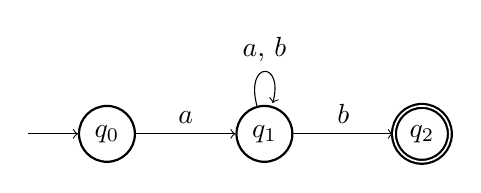
\begin{tikzpicture}
	\node[draw,circle] (q_0) at (0,0) {$q_0$};
	\node[draw,circle] (q_1) at (2,0) {$q_1$};
	\node[draw,circle,double] (q_2) at (4,0) {$q_2$};
	\draw[->] (-1,0) -- (q_0);
	\draw[->] (q_0) -- (q_1) node[midway,anchor=south] {$a$};
	\draw[->] (q_1) -- (q_2) node[midway,anchor=south] {$b$};
	\draw (q_1) edge [loop above] node {$a$, $b$} (q_1);
	\end{tikzpicture}
	\end{figure}
 	Bei Eingabe von $b$ im Zustand $q_1$ gibt es mehrere Möglichkeiten \vspace{0.5cm}
	
	(siehe Berechnungsbaum an der Tafel).
\end{frame}
\begin{frame}
	\frametitle{NEA: Aufgabe}
 Welche Sprache akzeptiert der nichtdeterministische endliche Automat
 zu dem folgenden Zustandsgraphen?
\begin{center}

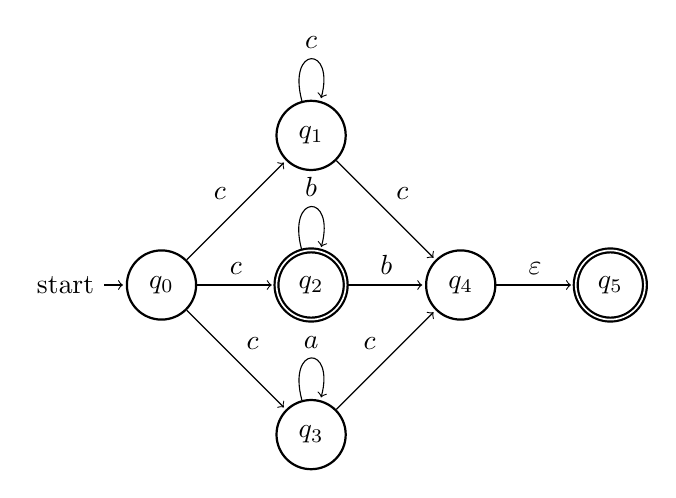
\begin{tikzpicture}[scale=0.6,node distance=1.9cm,shorten >=1pt,auto]
\node[state,initial]   (q_0)                {$q_0$};
\node[state,accepting]           (q_2) [right of=q_0]  {$q_2$};
\node[state] (q_1) [above of=q_2] {$q_1$};
\node[state] (q_3) [below of=q_2]  {$q_3$};
\node[state] (q_4) [right of=q_2]  {$q_4$};
\node[state,accepting] (q_5) [right of=q_4] {$q_5$};
\path[->]	(q_0) 	edge 			node {$c$} 		(q_1)
			edge 			node {$c$} 		(q_2)
			edge 			node {$c$} 		(q_3)
		(q_1)	edge [loop above]	node {$c$}		()
			edge 			node {$c$}		(q_4)
		(q_2)	edge [loop above]	node {$b$}		()
			edge 			node {$b$}		(q_4)
		(q_3)	edge [loop above]	node {$a$}		()
			edge			node {$c$}		(q_4)
	    (q_4)   edge        node {$\varepsilon$} (q_5);
\end{tikzpicture}
\end{center}
\end{frame}

\subsubsection{Potenzmengenkonstruktion}
\frame{
\frametitle{Potenzmengenkonstruktion}
Zu jedem nichtdeterministischen endlichen Automaten existiert ein äquivalenter deterministischer endlicher Automat.
 \begin{figure}[H]
 \begin{center}
 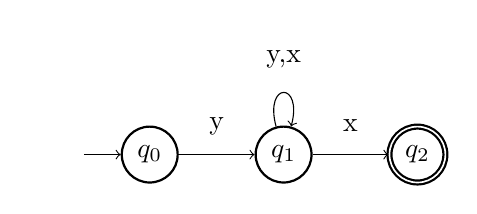
\begin{tikzpicture}[node distance=1.7cm]
 \tikzstyle{every node}=[circle, thick, minimum size = 7mm]
 \tikzstyle{normal}=[draw]
 \node[normal] 	(q0)		{$q_0$};
 \node[normal] 	(q1)	[right of=q0] {$q_1$};
 \node[normal,double]		(q2)	[right of=q1]{$q_2$};
 \node 		(s) 	[left of =q0, xshift=0.5cm]	{};
 
 \draw[->](s) to (q0);
 \draw[->](q0) to node[above]{y} (q1);
 \draw[->, loop above](q1) to node[above]{y,x} (q1);
 \draw[->](q1) to node[above]{x} (q2);x
 \end{tikzpicture}
 \end{center}
 \end{figure}
In eine Tabelle werden die Automatenzustände und ihre Folgezustände bei jeweiliger Eingabe eingetragen. \\
\begin{center}
\vspace{-6pt}
\begin{tabular}{l|l|l}
    & y & x \\
\hline
 $\{q_0\}$ 	&	 $\{q_1\}$	&	$\emptyset$ \\
 $\{q_1\}$	&	$\{q_1\}$	&	$\textcolor{red}{\{q_1, q2 \}}$\\
\end{tabular}
\end{center}
}
\frame{
\frametitle{Potenzmengenkonstruktion}
Ein \textcolor{red}{neuer Zustand} entsteht, wenn man von einem alten Zustand durch eine Eingabe in mehrere Zustände kommt.
\vspace{-0.3cm}
\begin{center}
\begin{tabular}{l|l|l}
    & y & x \\
\hline
 $\{q_0\}$ 	&	 $\{q_1\}$	&	$\emptyset$ \\
 $\{q_1\}$	&	$\{q_1\}$	&	$\textcolor{red}{\{q_1, q_2\}}$\\ \
 $\textcolor{red}{\{q_1, q_2\}}$ & 	$\{q_1\}$	&	$\{q_1, q_2\}$\\
 $\emptyset$	&	$\emptyset$		& 	$\emptyset$
\end{tabular}
\end{center}
\vspace{-1cm}
\begin{figure}[H]
\begin{center}
 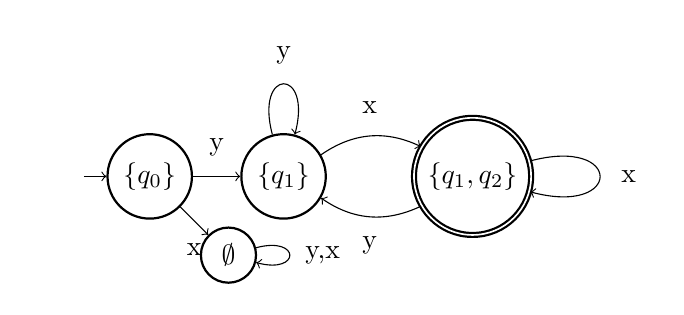
\begin{tikzpicture}[node distance=1.7cm]
 \tikzstyle{every node}=[circle, thick, minimum size = 7mm]
 \tikzstyle{normal}=[draw]
 \node[normal] 	(q0)		{\{$q_0$\}};
 \node[normal] 	(q1)	[right of=q0] {\{$q_1$\}};
 \node[normal,double,node distance=2.4cm]		(q2)	[right of=q1]{\{$q_1, q_2$\}};
 \node[normal]	(f) at (1,-1)	{$\emptyset$};
 \node 		(s) 	[left of =q0, xshift=0.5cm]	{};
  \draw[->](q0) to node[above]{y}(q1);
  \draw[->](s) to (q0);
  \draw[->](q0) to node[below]{x}(f);
  \draw[->,loop above](q1) to node[above]{y}(q1);
  \draw[->,bend left](q1) to node[above]{x}(q2);
  \draw[->, bend left](q2) to node[below]{y}(q1);
  \draw[->, loop right](q2) to node[right]{x}(q2);
  \draw[->, loop right](f) to node[right]{y,x}(f);
\end{tikzpicture}
\end{center}
\end{figure}

}
\frame{
\frametitle{Potenzmengenkonstruktion}
Die Einträge der ersten Spalte sind die neuen Zustände. Alle Mengen, die einen Endzustand enthalten, sind wiederum im neuen Automaten Endzustände.
\begin{figure}[H]
\begin{center}
 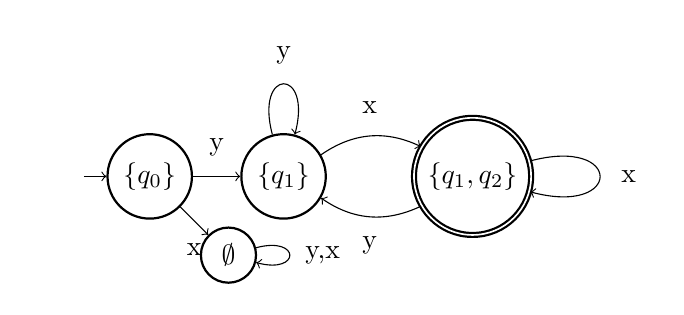
\begin{tikzpicture}[node distance=1.7cm]
 \tikzstyle{every node}=[circle, thick, minimum size = 7mm]
 \tikzstyle{normal}=[draw]
 \node[normal] 	(q0)		{\{$q_0$\}};
 \node[normal] 	(q1)	[right of=q0] {\{$q_1$\}};
 \node[normal,double,node distance=2.4cm]		(q2)	[right of=q1]{\{$q_1, q_2$\}};
 \node[normal]	(f) at (1,-1)	{$\emptyset$};
 \node 		(s) 	[left of =q0, xshift=0.5cm]	{};
  \draw[->](q0) to node[above]{y}(q1);
  \draw[->](s) to (q0);
  \draw[->](q0) to node[below]{x}(f);
  \draw[->,loop above](q1) to node[above]{y}(q1);
  \draw[->,bend left](q1) to node[above]{x}(q2);
  \draw[->, bend left](q2) to node[below]{y}(q1);
  \draw[->, loop right](q2) to node[right]{x}(q2);
  \draw[->, loop right](f) to node[right]{y,x}(f);
\end{tikzpicture}
\end{center}
\end{figure}

}
\subsection{Konstruktion eines DEA aus einem NEA}
\begin{frame}
  \frametitle{NEA2DEA: Aufgaben}
  Über dem Alphabet $\Sigma = \{a,b\}$ sei der reguläre
  Ausdruck
  $r := {(a \cup (ab (b)^* ba))^*}$
  gegeben.
  
  Geben Sie einen NEA an, der $L(r)$ erkennt. Begründen Sie
    kurz die Korrektheit Ihres Automaten, ein formaler
    Korrektheitsbeweis ist jedoch nicht erforderlich.\\
    (Hinweis: Es gibt einen NEA mit 3 Zuständen.)
\end{frame}


\begin{frame}
	\frametitle{Eliminierung von $\varepsilon$-Übergängen}
	\begin{block}{Satz 2.13 (Skript)}
	\begin{itemize}
	 \item Zu jedem nichtdeterministischen endlichen Automaten mit \(\varepsilon\)-Übergängen gibt es einen äquivalenten nichtdeterministischen
	 endlichen Automaten ohne \(\varepsilon\)-Übergänge, der nicht mehr Zustände hat.
	 \item äquivalent = akzeptiert die selbe Sprache.
	\end{itemize}
	\end{block}
	\begin{block}{Erinnerung}
		Der \(\varepsilon\)-Abschluss $E(q)$ eines Zustandes $q$ ist definiert als die Menge aller Zustände, die von $q$ aus durch lediglich \(\varepsilon\)-Übergänge erreichbar sind. ($q$ selbst zählt auch dazu)
	\end{block}
\end{frame}
\begin{frame}
\frametitle{Eliminierung von $\varepsilon$-Übergängen}
	\vspace{-0.9cm}
	\begin{block}{Konstruktion}
	Zu einem NEA \(A := (Q, \Sigma, \delta, s, F)\) mit \(\varepsilon\)-Übergängen konstruieren wir einen 
	  äquivalenten NEA \(\tilde{A} := (\tilde{Q}, \Sigma, \tilde{\delta}, \tilde{s}, \tilde{F})\) mit
	 \begin{itemize}
	 \item \(\tilde{Q} := Q\)
	 \item \(\tilde{s} := s\)
	 \item \(\tilde{F} := \{q|E(q)\cap F \neq \emptyset\}\)
	 \item \[\tilde{\delta}(q,a) := 
	 \begin{cases}
	  \{q\}			& \text{falls $a = \varepsilon$} \\
	 \delta(E(q),a)	& \text{sonst}
	 \end{cases}\]
	 \end{itemize}
	\end{block}
	\begin{block}{Eigenschaften von \(\tilde{A}\)}
	 \(L(\tilde{A}) = L(A)\), und \(|\tilde{Q}| = |Q|\).
	\end{block}

\end{frame}
\begin{frame}
	\frametitle{NEA2DEA: Aufgaben}
Gegeben sei der NEA ${\cal A}=(\{s,q,f\},\{a,b,c\},\delta,s,\{f\})$, wobei
die Übergangsfunktion $\delta$ gegeben ist durch:
\begin{center}
$\begin{array}{r|cccc}
&\varepsilon & a & b & c\\\hline
s & \{q,f\} & \emptyset & \{q\} &\{f\}\\
q &  \emptyset & \{s\} & \{f\} & \{s,q\}\\
f & \emptyset & \emptyset &  \emptyset &  \emptyset\\
\end{array}$
\end{center}
\begin{enumerate}
\item Geben Sie zu dem Automaten ${\cal A}$ den Übergangsgraphen an und eliminieren
Sie die $\varepsilon$-Übergänge.
\item Ermitteln Sie mittels Potenzmengenkonstruktion den zu ${\cal A}$ äquivalenten
DEA. Geben Sie hierbei die Übergangsfunktion tabellarisch an.
\end{enumerate}
\end{frame}
%\begin{frame}	
%\frametitle{Aufgaben zu \(\varepsilon\)-Übergängen}
%Sei $A=(Q,\Sigma, \delta, s, \{q_f\})$ ein NEA, derart, dass es keine zu $s$ hinführenden und keine von $q_f$ ausgehenden Übergänge gibt. Beschreiben Sie für jede der folgenden Modifikationen von A die akzeptierte Sprache als Modifikation von $L=L(A)$:
%\begin{enumerate}
%\item Der Automat, der aus A konstruiert wird, indem $\varepsilon$-Übergänge von $s$ zu jedem Zustand hinzugefügt werden, der von $s$ aus auf einem Pfad erreichbar ist, dessen Beschriftungen sowohl Symbole aus $\Sigma$ als auch $\varepsilon$ enthalten können.
%\item Der Automat, der aus A konstruiert wird, indem von jedem Zustand $\varepsilon$-Übergänge nach $q_f$ hinzugefügt werden, von dem aus $q_f$ auf irgendeinem Pfad erreichbar ist.
%\item Der Automat, der aus A konstruiert wird, indem die unter (1) und (2) geforderten Modifikationen ausgeführt werden.
%\end{enumerate}
%
%\end{frame}



%Pumpin' Lemma
\subsection{Pumpin' Lemma}
\begin{frame}
\frametitle{Pumping Lemma}
\begin{exampleblock}{Pumping Lemma}
Sei $L$ eine reguläre Sprache. Dann existiert eine Zahl $n \in \mathbb{N}$, so dass für jedes Wort $w \in L$ mit $\left|w \right| > n$ eine Darstellung $$w = uvx$$ existiert, so dass folgende Eigenschaften erfüllt sind:

\begin{enumerate}
\item $v \neq \varepsilon$ 
\item $\left|uv\right| \leq n$ 
\item Für alle $i \in \mathbb{N}_0$ gilt: $uv^ix \in L$
\end{enumerate}
\end{exampleblock}

\begin{center}
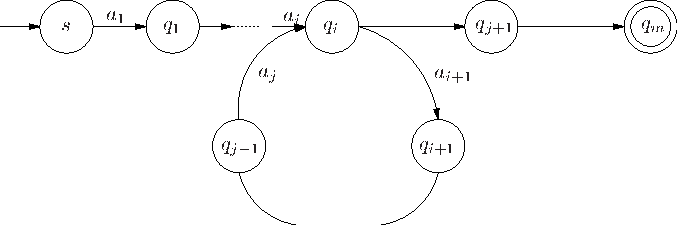
\includegraphics[width=0.55\textwidth]{images/Q116}
\end{center}

\end{frame}

\begin{frame}
\frametitle{Pumping Lemma: Übersicht}
\begin{itemize}
\item Jede reguläre Sprache erfüllt das Pumping Lemma. Aber: Nicht jede Sprache, die das Pumping Lemma erfüllt, ist regulär!
\item In der Übung wird üblicherweise die Kontraposition des Pumping-Lemmas verwendet: Man zeigt für eine Sprache, dass das Pumping-Lemma \emph{nicht} erfüllt ist, woraus folgt, dass diese Sprache \emph{nicht} regulär sein kann.

\pause\item $ \neg\left[ \exists n \in \N \,:\, \forall w \in L, |w| > n \,:\, \exists uvx=w \,:\, \ldots \forall i \in \N \,:\, uv^i x \in L\right] $ \\ $ \Leftrightarrow \forall n \in \N \,:\, \exists w \in L, |w| > n \,:\, \forall uvx=w \,:\, \ldots \exists i \in \N \,:\, uv^i x \not\in L $

\pause\begin{itemize}
\item Finden wir für \emph{jedes} $n$ \emph{ein} $w$ mit $\left|w\right| > n$, so dass für \emph{jede} Darstellung $w = uvx$ mit $v \neq \varepsilon$ sowie $\left|uv\right| \leq n$ ein $i \in \mathbb{N}_0$ existiert mit $uv^ix \notin L$, dann ist $L$ nicht regulär.
\end{itemize}
\end{itemize}

\end{frame}

\begin{frame}
\frametitle{Beispiel}
Sei $\Sigma = \{a, b\}$ und $L = \{a^nb^n\,|\,n\geq0\}$. (Also $L = \{\varepsilon,ab, aabb, aaabbb, \ldots\}$)
\begin{enumerate}
\item Angenommen, $L$ sei regulär. Sei dann $n$ wie im Pumping Lemma.
\item Wähle das Wort $w = a^nb^n$.
\item Es ist also $\left|w\right| > n$.
\item Nun ist aber für \emph{jede} Darstellung $w = uvx$ mit $\left|uv\right| \leq n$ und $v \neq \varepsilon$ $v = a^m$ mit $m \geq 0$. Demnach ist $uv^0x = a^lb^n \neq L$, da $l < n$.
\item Daher kann $L$ nicht regulär sein.
\end{enumerate}

\end{frame}

\begin{frame}
\frametitle{Pumping Lemma: Aufgaben}
Welche der folgenden Sprachen sind regulär? Begründen Sie Ihre Antwort.

\begin{enumerate}
\item $L=\{a^kc^lb^k \mid k, l \geq 0 \}$
\item Die Menge aller Wörter über $\{0, 1\}$, sodass auf jede Null eine Eins folgt
\item Die Menge der Wörter über $\{0, 1\}$, die die Form $w\bar{w}$ haben, wobei $\bar{w}$ aus $w$ gebildet
wird, indem alle Nullen durch Einsen und alle Einsen durch Nullen ersetzt werden; so ist etwa 
$\overline{011}=100$ und $011100$ ein Beispiel für ein Wort dieser Sprache
\end{enumerate}

\end{frame}

\subsection{Konstruktion eines regulären Ausdrucks}
\begin{frame}
\frametitle{Konstruktion eines RA aus einem DEA}
Wir wissen: Zu jedem DEA gibt es einen regulären Ausdruck, der genau die Sprache beschreibt, die der Automat akzeptiert. Wie konstruiert man nun diesen RA aus dem DEA?\\[0.6cm]
\textbf{Idee:} Betrachte die Sprachen $L_{q_r,i,q_t}$, definiert als \( w \in \Sigma^*\) mit $w$ überführt $q_r$ in $q_t$ unter Benutzung der Zwischenzustände $\{q_1,\ldots,q_i\}$
\begin{itemize}
\item Es ist $L = \cup_{f\in F} L_{s,n,f}$
\item Es ist weiterhin $L_{q_r,i+1,q_t} = L_{q_r,i,q_t} \cup (L_{q_r,i,q_{i+1}}(L_{q_{i+1},i,q_{i+1}})^*L_{q_{i+1},i,q_t})$
\item Letztlich ist $L_{q_r, 0, q_t}$ immer regulär, das sind die Zeichen mit denen man von $q_r$ nach $q_t$ kommt, ohne weitere Zustände zu verwenden (sowie $\varepsilon$ falls $r = t$).
\item Unter Benutzung dieser Punkte kann man nun einen Regulären Ausdruck zu einem DEA Konstruieren.
\end{itemize}
\end{frame}
\begin{frame}
\frametitle{Beispiele zum Verständnis}
\vspace{-1cm}
\begin{figure}[H]
\begin{center}
\begin{tikzpicture}[scale=0.6,node distance=1.9cm,shorten >=1pt,auto]
\node[state,initial]   (q_1)                {$q_1$};
\node[state,accepting] (q_2) [right of=q_0] {$q_2$};
\path[->]	(q_1) 	edge 			node {$0$} 		(q_2)
			edge [loop above]	node {$1$}		()
		(q_2)	edge [loop above]	node {$0$,$1$}		();
\end{tikzpicture}
\end{center}
\end{figure}
Was sind hier jeweils:
\begin{itemize}
\item $L_{q_1,0,q_1}$\pause $ = (1\cup\varepsilon)$
\item $L_{q_1,0,q_2}$\pause $ = (0)$
\item $L_{q_1,1,q_1}$\pause $ = (1^*)$
\item $L_{q_2,1,q_2}$\pause $ = (0\cup1\cup\varepsilon)$
\item $L_{q_2,2,q_2}$\pause $ = (0\cup1)^*$
\item $L_{q_1,2,q_2}$\pause $ = 1^*0(0\cup1)^*$
\end{itemize}
\end{frame}

\begin{frame}
\frametitle{Ausführliche Konstruktion}
\vspace{-1cm}
\begin{figure}[H]
\begin{center}
\begin{tikzpicture}[scale=0.6,node distance=1.9cm,shorten >=1pt,auto]
\node[state,initial]   (q_1)                {$q_1$};
\node[state,accepting] (q_2) [right of=q_0] {$q_2$};
\path[->]	(q_1) 	edge 			node {$0$} 		(q_2)
			edge [loop above]	node {$1$}		()
		(q_2)	edge [loop above]	node {$0$,$1$}		();
\end{tikzpicture}
\end{center}
\end{figure}
\begin{enumerate}
\item $L_{q_1,2,q_2} = L_{q_1,1,q_2}\cup(L_{q_1,1,q_2}(L_{q_2,1,q_2})^*L_{q_2,1,q_2})$
\item $L_{q_1,1,q_2} = L_{q_1,0,q_2}\cup(L_{q_1,0,q_1}(L_{q_1,0,q_1})^*L_{q_1,0,q_2}) = 0\cup((1\cup\varepsilon)(1\cup\varepsilon)^*0)$
\item $L_{q_2,1,q_2} = L_{q_2,0,q_2}\cup(L_{q_2,0,q_1}(L_{q_1,0,q_1})^*L_{q_1,0,q_2})$ $ = (0\cup1\cup\varepsilon)$
\item Also: $L_{q_1,2,q_2} = 0\cup(1\cup\varepsilon)(1\cup\varepsilon)^*0\cup((0\cup((1\cup\varepsilon)(1\cup\varepsilon)^*0))(0\cup1\cup\varepsilon)^*(0\cup1\cup\varepsilon))$
\item Vereinfacht: $1^*0(0\cup1)^*$
\end{enumerate}
\end{frame}

\begin{frame}[t]
\frametitle{Aufgabe}
Bestimmen Sie  mit dem im Beweis von Satz 2.14 verwendeten Verfahren die 
reguläre Sprache, die folgender deterministische endliche Automat erkennt:
\begin{figure}[H]
\begin{center}
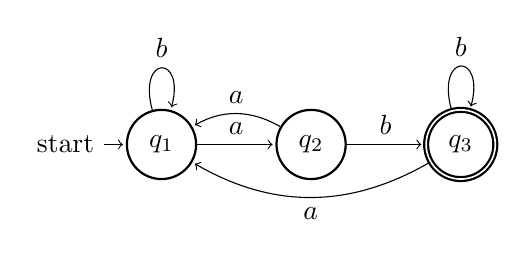
\begin{tikzpicture}[scale=0.6,node distance=1.9cm,shorten >=1pt,auto]
\node[state,initial]   (q_1)                {$q_1$};
\node[state] (q_2) [right of=q_1] {$q_2$};
\node[state,accepting] (q_3) [right of=q_2] {$q_3$};

\path[->]	(q_1) 	edge 			node {$a$} 		(q_2)
			edge [loop above]	node {$b$}		()
		(q_2)	edge [bend right]	node [above] {$a$}		(q_1)
			edge 			node {$b$}		(q_3)
		(q_3)	edge [loop above]	node {$b$}		()
			edge [bend left]	node {$a$}		(q_1);
\end{tikzpicture}
\end{center}
\end{figure}
\end{frame}

\begin{frame}
\frametitle{Bis zum nächsten Mal!}
\begin{center}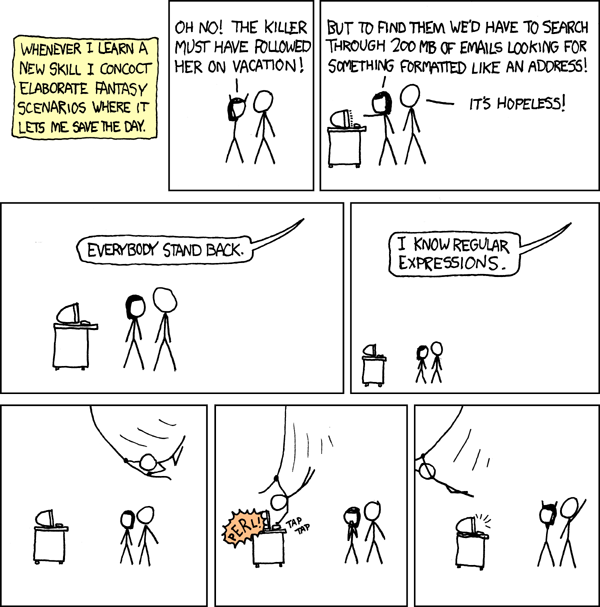
\includegraphics[height=0.6\textheight]{images/regular_expressions.png}\end{center}
\vspace{-0.5cm}

\small{\begin{quote}
Some people, when confronted with a problem, think "I know, I'll use regular expressions." Now they have two problems. -- Jamie Zawinski
\end{quote}}

\end{frame}

\frame{
  \frametitle{Lizenzen}
  \center
  \includegraphics[width=2em]{images/by}
  \includegraphics[width=2em]{images/cc}
  \includegraphics[width=2em]{images/sa}
  \\
  {\tiny

Dieses Werk ist unter einem ``Creative Commons Namensnennung-Weitergabe unter gleichen Bedingungen 3.0 Deutschland``-Lizenzvertrag lizenziert. Um eine Kopie der Lizenz zu erhalten, gehen Sie bitte zu \href{http://creativecommons.org/licenses/by-sa/3.0/de/}{http://creativecommons.org/licenses/by-sa/3.0/de/} oder schreiben Sie an Creative Commons, 171 Second Street, Suite 300, San Francisco, California 94105, USA.\\
  \vspace{1cm}
  Davon ausgenommen sind das Titelbild, welches aus der März-April 2002 Ausgabe von American Scientist erschienen ist und ohne Erlaubnis verwendet wird, sowie das KIT Beamer Theme. Hierfür gelten die Bestimmungen der jeweiligen Urheber.
  \vspace{1cm}
  \\ 
  }
  %Habe hier die Reihenfolge etwas umgestellt, weil die Formatierung bei mir komisch aussah. 
  %Wenn es bei dir anders ist, kannst du es auch wieder zurückändern, dann haben wir unterschiedliche Kompilieroptionen
}

\end{document}